\section{Практична частина}
\setlength{\parindent}{4em}
\begin{center}
  {\textbf{\emph{Визначення концентрації розчину за допомогою коефіціента заломлення}}}
\end{center}
\begin{figure}[ht]

\centering

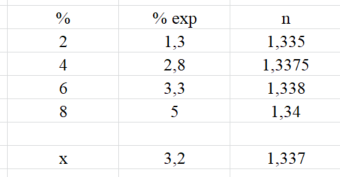
\includegraphics[width=0.55\linewidth]{Pics/table1.png}

\label{table1}

\end{figure}
\begin{figure}[ht]

\centering

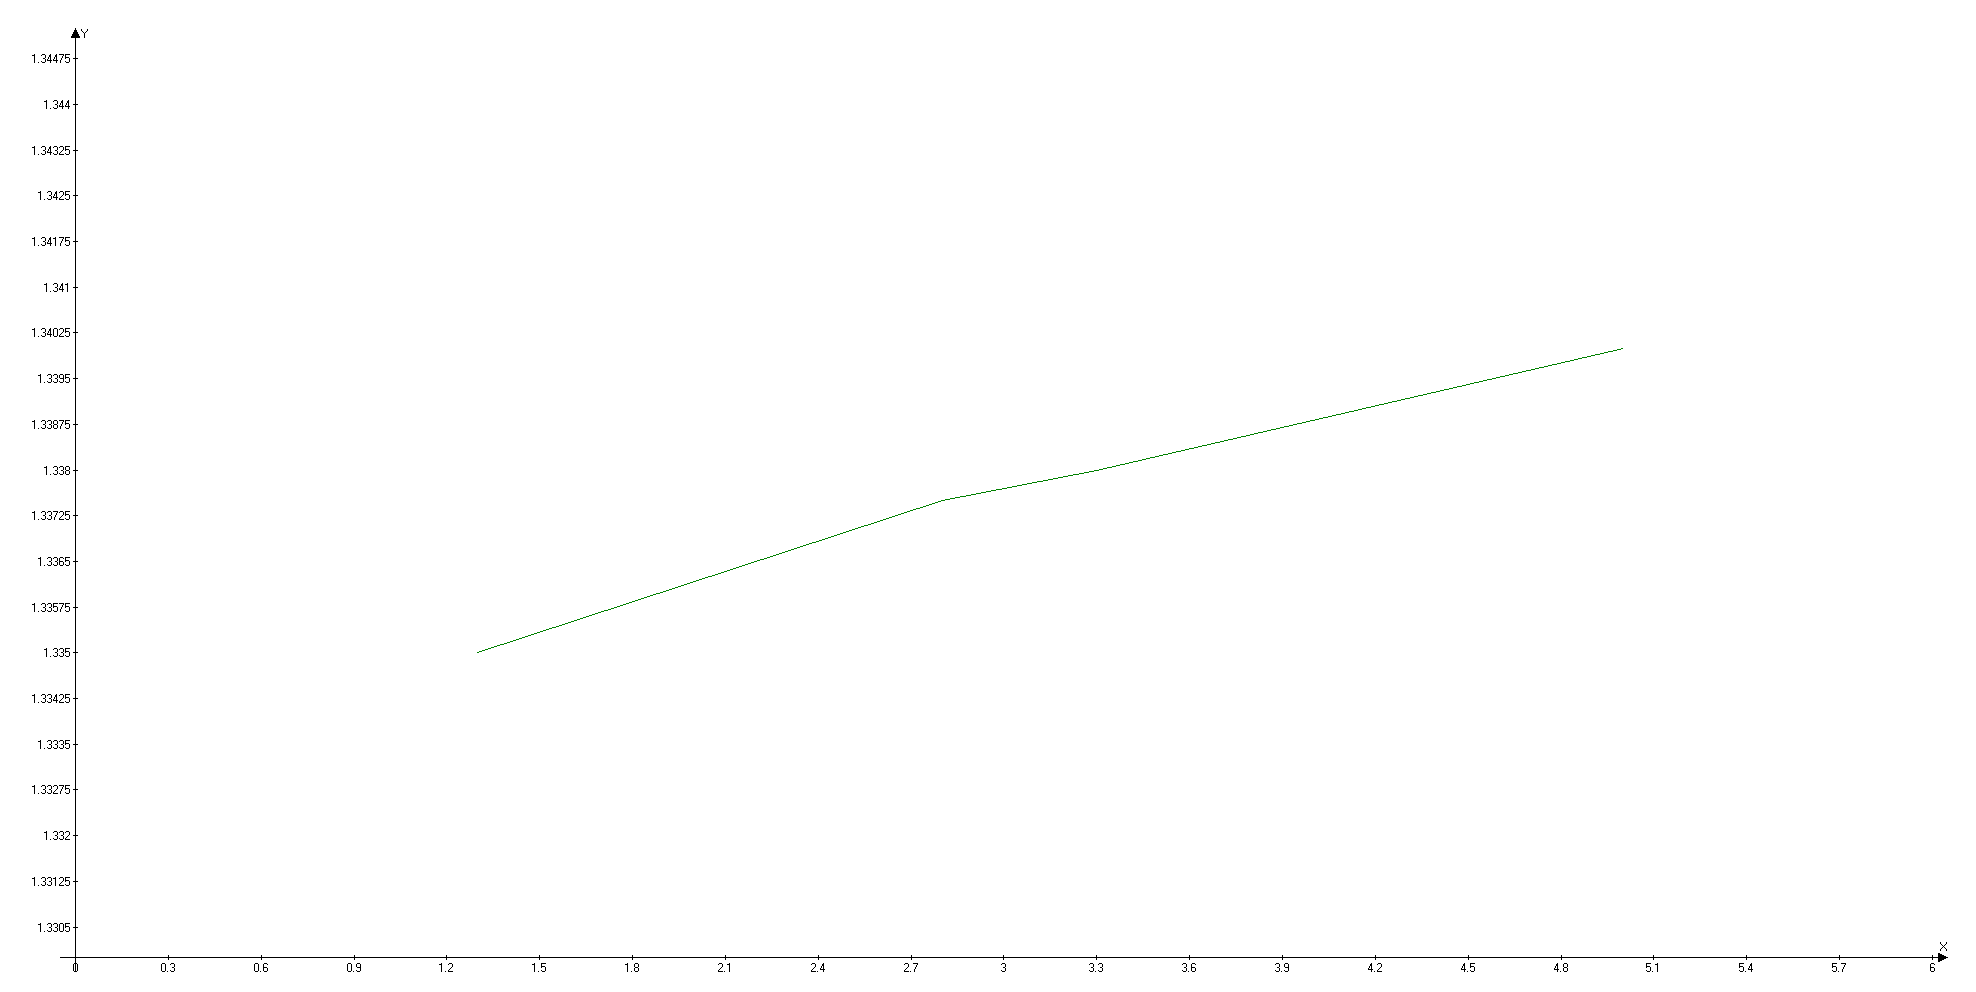
\includegraphics[width=0.7\linewidth]{Pics/Plot1.png}

\label{table1}

\end{figure}
\qquad З графіку можно побачити, що коефіціенту заломлення відповідає концентрація $\approx$ 3,1. Експериментально визначена концентрація розчину: 3,2. Теоретичне відхилення: $\epsilon = \frac{3,2-3,1}{3,1} = 3\%$
\begin{center}
  {\textbf{\emph{Визначення питомої рефракції }}}
\end{center}
Робоча формула:
$$R = \frac{n^2 -1}{n^2 + 1} \cdot \frac{1}{\rho}$$
\begin{figure}[ht]

\centering

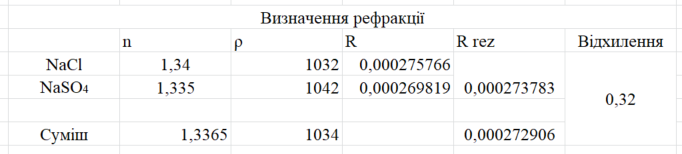
\includegraphics[width=1\linewidth]{Pics/table2.png}


\label{Prac2}

\end{figure}
